\chapter{Implementation in {\sc JKind}}
\label{ch:impl}

\newcommand{\jkind}{\texttt{JKind}\xspace}
\newcommand{\kind}{\texttt{Kind}\xspace}
\newcommand{\jkindapi}{\texttt{JKindApi}\xspace}
\newcommand{\lustre}{\texttt{Lustre}\xspace}
\newcommand{\spear}{\texttt{SpeAR}\xspace}
\newcommand{\simpal}{\texttt{SIMPAL}\xspace}
\newcommand{\limp}{\texttt{Limp}\xspace}
\newcommand{\agree}{\texttt{AGREE}\xspace}
\newcommand{\gryphon}{\texttt{Gryphon}\xspace}

\renewcommand{\paragraph}[1]{\vspace{5pt}\noindent {\bf #1}}
\newcommand{\application}[2]{
  \paragraph{#1} \hfill {\it #2}
  \vspace{1pt}
}



This chapter explains the implementation of IVC techniques. Part of this chapter is from a collaborative paper with Gacek et al. \cite{jkindpaper} and ~\cite{jkind}.

All of the inductive validity core algorithms presented in Chapter \ref{ch:ivc} have been implemented in \texttt{JKind} model checker ~\cite{jkind}. \jkind is an
open-source industrial
infinite-state inductive model checker for safety properties. Models
and properties in \jkind are specified in
\lustre~\cite{halbwachs1991ieee}, a synchronous data-flow language,
using the theories of linear real and integer arithmetic. \jkind uses
SMT-solvers to prove and falsify multiple properties in parallel.

\jkind is one of a number of similar infinite-state inductive model
checkers including {\sc Kind 2}, \kind, {\sc NuXmv}, and {\sc
  Zustre}. These tools each offer multi-engine solvers that utilize
both k-induction and some variant of IC3/PDR. In a recent
comparison~\cite{champion2016cav}, \jkind was the second most capable
solver in terms of the number of problems solved (behind {\sc Kind 2})
and had competitive performance across a large benchmark suite. The
most noticeable bottleneck in \jkind is the start-up time for the Java
Virtual Machine (JVM). This cost is insignificant for larger models
but causes decreased performance for benchmarks consisting of many
very small models.
There are also other tools such as \texttt{ESBMC-DepthK} \cite{rocha2017model},  \texttt{VVT} \cite{beyer2016smt} \texttt{CPAchecker}, \cite{beyer2015boosting}, \texttt{CPROVER} \cite{brain2015safety} attempting to prove C programs using similar techniques ($k$-induction, invariant generation, and PDR).

An important characteristic of \jkind is that is it designed to be integrated directly into user-facing applications. Written in Java, \jkind runs on all major platforms and is easily compiled into other Java applications. \jkind bundles the Java-based \texttt{SMTInterpol} solver~\cite{Christ2012:SMTInterpol} and has no external dependencies. However, it can optionally call
\texttt{Z3}~\cite{DeMoura08:z3},
\texttt{Yices}~\cite{Dutertre06:yices}, \texttt{MathSAT}~\cite{Cimatti2013:MathSAT}, and \texttt{CVC4} \cite{barrett2011cvc4} if they are available.

Another distinguishing characteristic of \jkind is its focus on the usability  of results. For a falsified property, \jkind provides options for simplifying the
counterexample in order to highlight the root cause of the failure. New integration of IVCs in \jkind , allows it to provide traceability between the property and individual model elements for a proven property. These additional usability aspects have been found in industrial applications to be at least as important as the primary results \cite{jkindpaper}.

In the rest of this chapter, we describe \jkind architecture, functionality, and applications. Then, we provide implementation details about the integration of IVCs in this tool.


\section{{\sc JKind} Functionality and Main Features}

\begin{figure}
  \centering
  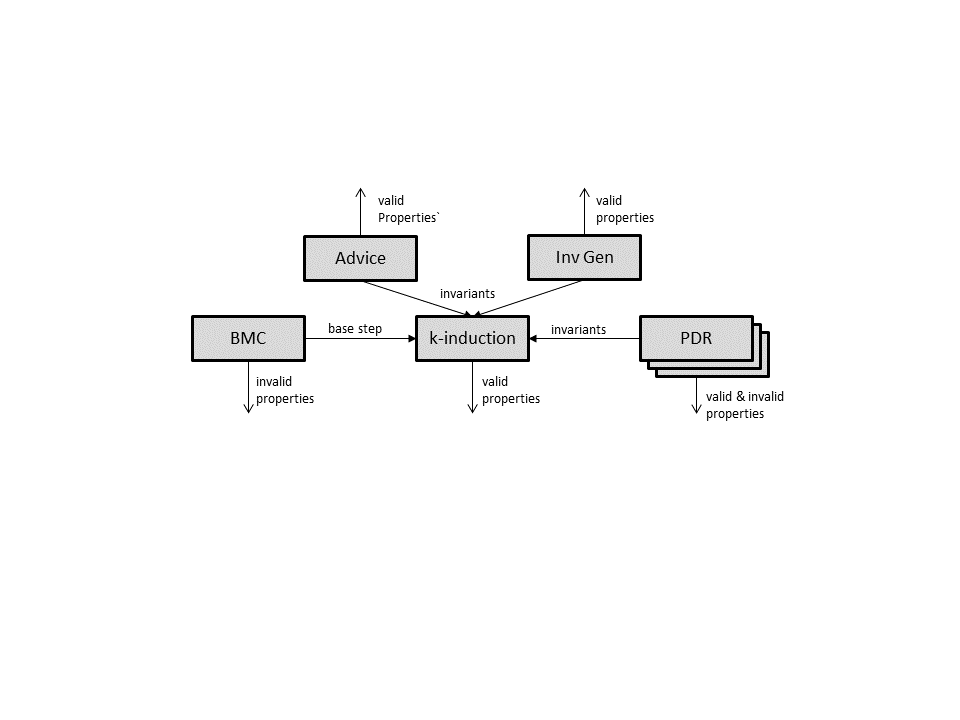
\includegraphics[width=\textwidth]{engines.png}

  \caption{\jkind engine architecture}
  %\vspace{-1em}
 % \mike{Shrink figure vertically}
  \label{fig:engines}
\end{figure}

\jkind is structured as several parallel engines that coordinate to
prove properties, mimicking the design of \kind\ and \kind\ 2~\cite{champion2016cav, kahsai2011pdmc}.
Some engines are directly responsible for proving properties, others aid that effort by generating invariants, and still others are reserved for post-processing of proof or counterexample results. Each engine can be enabled or disabled separately based on the user's needs. The architecture of \jkind allows any engine to broadcast information to the other engines (for example, lemmas, frames, proofs/counterexamples) allowing straightforward integration of new functionality.

The solving engines in \jkind are:

\begin{itemize}
  \item \textbf{Bounded Model Checking (BMC).} The BMC engine performs a standard iterative unrolling of the transition relation to find counterexamples and to serve as the base case of $k$-induction. The BMC engine guarantees that any counterexample it finds is minimal in length.
  \item \textbf{$k$-induction.} The $k$-induction engine performs the inductive step of $k$-induction, possibly using invariants generated by other engines. \textbf{Invariant Generation.} The invariant generation engine uses a template-based invariant generation technique~\cite{kahsai2012nfm} using its own $k$-induction loop.
  \item \textbf{Property Directed Reachability (PDR).} The PDR engine performs property directed reachability~\cite{een2011fmcad} using the implicit abstraction technique~\cite{cimatti2014tacas}. Unlike BMC and $k$-induction, each property is handled separately by a different PDR sub-engine. Invariants generated as a side-product of PDR are shared with the $k$-induction process.
\end{itemize}

Invariant sharing between the solvers (shown in Figure~\ref{fig:engines}) is an important part of the architecture.  In our internal benchmarking, we have found that implicit abstraction PDR performs best when operating over a single property at a time and without use of lemmas generated by other approaches.  On the other hand, the invariants generated by PDR and template lemma generation often allow k-induction, which operates on all properties in parallel, to substantially reduce the verification time required for models with large numbers of properties.  %As described in Section~\ref{sec:benchmarks}, \jkind\ is competitive with other tools

\subsection{Post Processing and Re-verification}

A significant part of the research and development effort for \jkind\ has focused on
post-processing results for presentation and repeated verification of models under development.

%and supporting re-verification of slightly-modified models.  Simplifying counterexamples to support root-cause analysis and providing traceability information to automatically create traceability matrices and determine adequacy of requirements has been important in the industrial use of the tools.  Additionally, this type of coverage and traceability information is often required for certification of safety critical systems~\cite{DO178C}.  To support these uses,


\subsubsection{Smoothing}

To aid in counterexample understanding and in creating structural coverage tests that can be more easily explained, \jkind\ provides an optional post-processing step to minimize the number of changes to input variables, {\em smoothing} the counterexample.
The smoothing engine uses a \texttt{MaxSat} query over
the original BMC-style unrolling of the transition relation combined
with weighted assertions that each input variable does not change on
each step. The \texttt{MaxSat} query therefore tries (as best as
possible) to hold all inputs constant while still falsifying the
original property. This engine is only available with SMT-solvers that
support \texttt{MaxSat} such as \texttt{Yices} and \texttt{Z3}.

\subsubsection{Advice}

The advice engine saves and re-uses the invariants that were used by \jkind to prove the properties of a model.  Prior to analysis, \jkind\ performs model slicing and flattening to generate a flat transition-relation model.  Internally, invariants are stored as a set of proven formulas (in the \lustre syntax) over the variables in the flattened model.  An {\em advice} file is simply the emitted set of these invariant formulas.  When a model is loaded, the formulas are loaded into memory; formulas that are no longer syntactically or type correct are discarded, and the remaining set of formulas are submitted as an initial set of possible invariants to be proved via $k$-induction: if they are proved, they are passed along to other engines; if falsified, they are discarded.
%
Names constructed between multiple runs of \jkind\ are stable, so if a model is unchanged, it can be trivially re-proved using the invariants and k-induction with $k=1$.  In the case that a model is a small delta of a previously-proved model, it is often the case that most of the invariants can be re-proved, leading to reduced verification times.

\section{Tool Installation}
The prerequisite for installing and using JKind is to have Java installed and on the PATH variable for the OS.
Installing JKind is accomplished by the following steps:
\begin{enumerate}
  \item Download the zip containing the latest release from:
  
   https://github.com/agacek/jkind/releases 
   
   As of the writing of this document, that is version 4.0.\footnote{All IVCs techniques are not yet part of the official release, but they can be obtained from \cite{mygit}}
  \item Unzip the contents of that zip to the directory of your choice.
  \item Add the folder from step 2 to the PATH variable for your OS.
The installation can be tested by executing jkind –help from the command line.
\end{enumerate}
Successful installation will provide the following result in Figure \ref{fig:jkins}.

 \begin{figure}
 \centering
  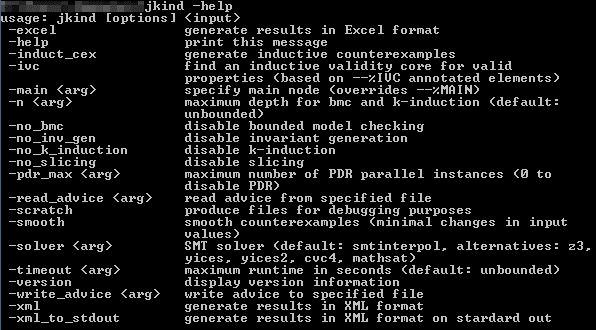
\includegraphics[width=\columnwidth]{figs/jkindcon.png}
  %\vspace{-0.1in}
  \caption{Successful installation of \texttt{JKind}}
  \vspace{0.1in}
  \label{fig:jkins}
\end{figure}

To add a solver, users must perform these steps:
\begin{enumerate}
  \item Download the solver of choice.
  \item Unzip the contents of the solver into a directory.
  \item Create an environment variable called $<$SOLVER$>$\_HOME that points to the directory used the previous step. This is:
      \begin{itemize}
        \item CVC4\_HOME for \texttt{CVC4}
        \item Z3\_HOME for \texttt{Z3}
        \item MATHSAT\_HOME for \texttt{MathSAT}
        \item YICES\_HOME for \texttt{Yices 1}
        \item YICES2\_HOME for \texttt{Yices 2}
      \end{itemize}
  \item \jkind will automatically look for the ``bin'' directory under $<$SOLVER$>$\_HOME when the solver is activated.
\end{enumerate}


\section{{\sc JKind} Lustre Grammar and Command Line Arguments}
\jkind accepts input from the synchronous dataflow language Lustre used for programming real-time systems. A dataflow language consists of a set of equations that assign variables where a variable can be computed as soon as its data dependencies have been computed. Such a language is a completely functional model without side effects, suitable for formal verification and program transformation. Like all functional language, a data flow language is naturally parallel where the only constraints on parallelism are due to the data-dependencies between variables.

Dataflow models can be either synchronous or asynchronous. In a synchronous dataflow model, the model is recomputed in a sequence of time instants. In an asynchronous model, the outputs of the system are continually recomputed depending on the inputs to the system.

\subsection{Syntax Overview}
\jkind Lustre grammar is built in \texttt{ANTLR} and can be referenced at
\emph{http://github.com/agacek/\\jkind/blob/master/jkind-common/src/jkind/lustre/parsing/Lustre.gz}.

\jkind supports single line and multi-line comment styles. The grammar elements for comments are shown in Figure \ref{fig:jk1}.

 \begin{figure}
 \centering
  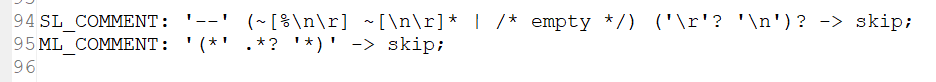
\includegraphics[width=\textwidth]{figs/jk1.png}
  %\vspace{-0.1in}
  \caption{\texttt{Jkind} comment grammar elements}
  \vspace{0.1in}
  \label{fig:jk1}
\end{figure}

The grammar for identifiers in \texttt{Jkind} are shown in Figure \ref{fig:jk2}. Valid identifers will begin with a upper or lowercase letter, followed by 0 or more letters, numbers, or underscore characters.

 \begin{figure}
 \centering
  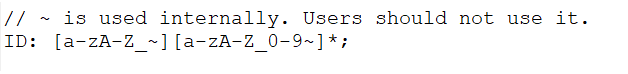
\includegraphics[width=0.75\textwidth]{figs/jk2.png}
  %\vspace{-0.1in}
  \caption{\texttt{Jkind} identifier grammar}
  \vspace{0.1in}
  \label{fig:jk2}
\end{figure}

The grammar for \texttt{Jkind} literals are shown in Figure \ref{fig:jk3}.

 \begin{figure}
 \centering
  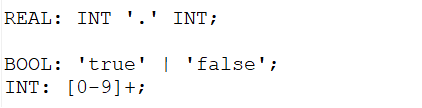
\includegraphics[width=0.5\textwidth]{figs/jk3.png}
  %\vspace{-0.1in}
  \caption{\texttt{Jkind} literal grammar}
  \vspace{0.1in}
  \label{fig:jk3}
\end{figure}

A Lustre program is a collection of constant, type, node, and function declarations. The grammar elements for these declarations are shown in Figure \ref{fig:jk4}.

 \begin{figure}
 \centering
  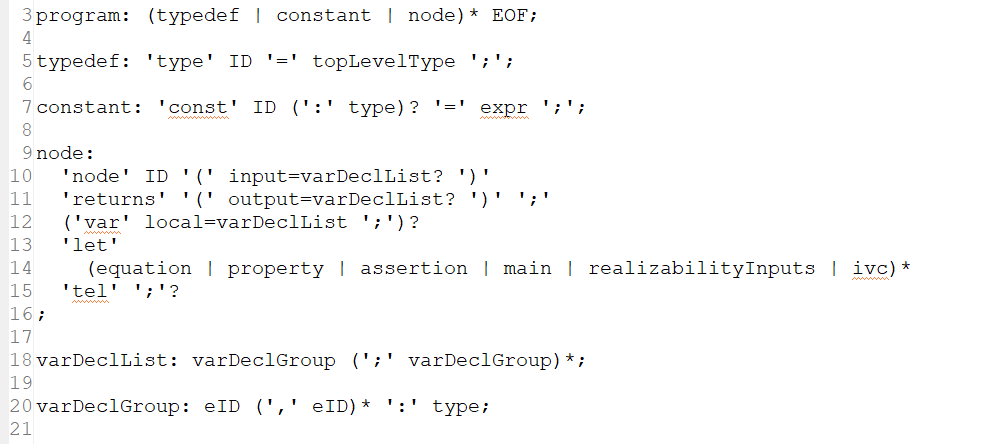
\includegraphics[width=\textwidth]{figs/jk4.png}
  %\vspace{-0.1in}
  \caption{Lustre program declarations}
  \vspace{0.1in}
  \label{fig:jk4}
\end{figure}


\jkind performs different analyses such as realizability, IVCs, and safety verification, etc. based on several LUSTRE annotations shown in Figure \ref{fig:jk7}.  The entry point of \jkind analysis is a node. For the programs with more than one node,  the node annotated with the $-$$-\%$MAIN declaration is considered as the entry point, otherwise \jkind will use the last node in the file as the main node. To do any meaningful analysis, a Lustre program must have at least one node defined. The remaining elements (constants, type definitions, and functions) can be used to specify a Lustre program for analysis. Properties are Lustre equations identified with $-$$-\%$PROPERTY annotation. \jkind runs the verification engines over equations listed in this annotation. We have added one more annotation for IVC analyses, $-$$-\%$IVC, which will be described in the next section.

 \begin{figure}
 \centering
  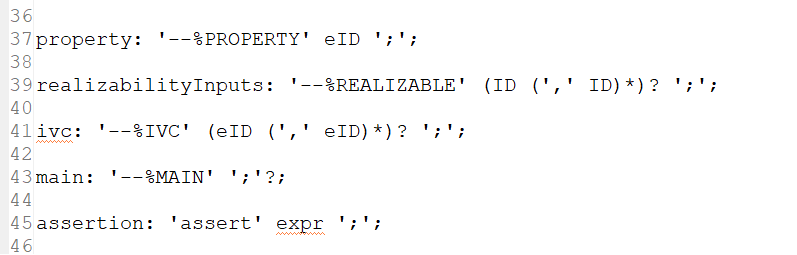
\includegraphics[width=0.8\textwidth]{figs/jk7.png}
  %\vspace{-0.1in}
  \caption{Lustre annotations used by \jkind}
  \vspace{0.1in}
  \label{fig:jk7}
\end{figure}

 \begin{figure}
 \centering
  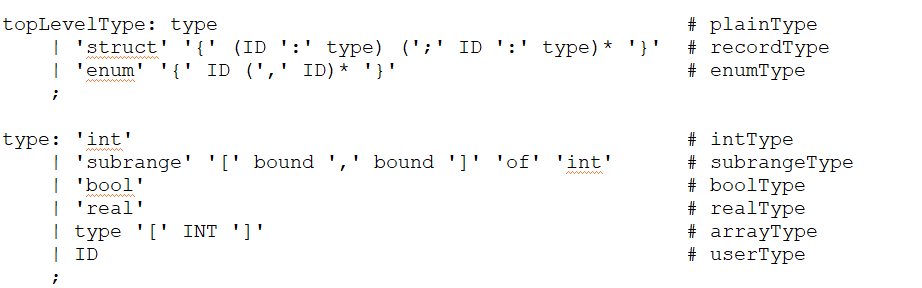
\includegraphics[width=\textwidth]{figs/jk5.png}
  %\vspace{-0.1in}
  \caption{\jkind Lustre type grammar}
  \vspace{0.1in}
  \label{fig:jk5}
\end{figure}

Figure \ref{fig:jk5} shows the grammar elements for the Lustre types that \jkind supports. The grammar snippet in Figure \ref{fig:jk6} shows the Lustre expressions elements \jkind supports. ID expressions are used to reference variables, enumeration values, and record field elements by name. Literal expressions are used to express boolean literals of true/false, integer literals 0 to Infinity, and real literals 0.0 to Infinity. For more information on other expressions, see \jkind User Guide \cite{jkind}.

\begin{figure}
 \centering
  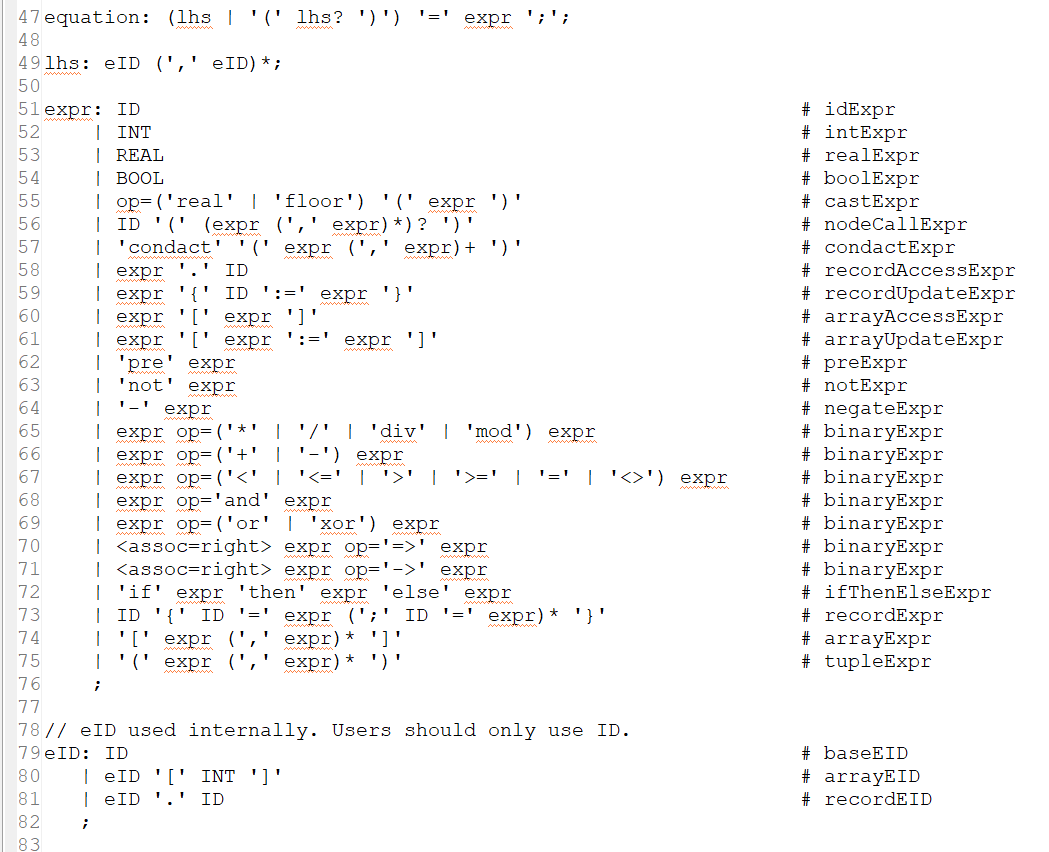
\includegraphics[width=\textwidth]{figs/jk6.png}
  %\vspace{-0.1in}
  \caption{\jkind Expression and Equation grammar}
  \vspace{0.1in}
  \label{fig:jk6}
\end{figure}

\subsection{Command Line}
Different \jkind functionalities explained so far are accessible from the tool command line. Table \ref{tab:jkindcm} summarizes major options in \jkind.

\begin{table}
  \caption{Major options in \jkind command line}
   \vspace{-0.1in}
  \centering
\begin{tabularx}{\linewidth}{|c|L|}
\hline
    Command & Description\\
  \hline\hline
  % after \\: \hline or \cline{col1-col2} \cline{col3-col4} ...
  \small{$-solver $ $<$$arg$$>$} & \small{SMT solver (default: smtinterpol, alternatives: z3, yices, yices2, cvc4, mathsat)}\\[0.1ex]\hline
  \small{$-n $ $<$$arg$$>$ } & \small{maximum depth for BMC and $k$-induction} \\[0.1ex]
 \small{ $-timeout $ $<$$arg$$>$ }& \small{maximum runtime in seconds (default: unbounded)}\\[0.1ex]\hline
  \small{$-no\_bmc$} & \small{disable bounded model checking} \\
  \small{$-no\_k\_induction $} & \small{ disable $k$-induction} \\
  \small{$-pdr\_max$ $<$$arg$$>$} &\small{ maximum number of PDR parallel instances: if $arg$ is 0, PDR will be disabled} \\[0.1ex]
  \small{$-no\_inv\_gen $} & \small{disable invariant generation} \\
  \small{$-no\_slicing $} & \small{disable slicing} \\[0.1ex]\hline
  \small{$-ivc$ }& \small{find an inductive validity core for valid properties (based on $--\%IVC$ annotated  elements in the LUSTRE input file)} \\
  \small{$-all\_assigned$} & \small{mark all equations of the input file as $--\%IVC$} \\
  \small{$-all\_ivcs$} & \small{find all inductive validity cores for valid  properties}\\
  \small{$-all\_ivcs\_algv$ $<$$arg$$>$ }& \small{algorithm to be used for finding all IVCs (1: offline generation, 2: online generation)} \\
  %\small{$-all\_ivcs\_max\_grows$ $<$$arg$$>$} & \small{used with the previous option while $arg = 2$ to specify maximal number of grows in the map-based  shrinking procedure (in MIVC enumeration algorithms)} \\[0.5ex]
  \small{$-bvc$ }& \small{generate BVC at depth $-n$ within given $-timeout$} \\
  \small{$-use\_unsat\_core$ $<$$arg$$>$ }& \small{call UCBF algorithm on an input xml file containing the result provided by the use of $-ivc$ and $-xml$ options}\\[0.1ex]\hline
  \small{$-xml$} & \small{generate results in XML format}\\
  \small{$-scratch$} & \small{produce files for debugging purposes}\\[0.1ex]\hline
    \small{$-write\_advice$ $<$$arg$$>$} & \small{write advice to specified file}\\
  \small{$-read\_advice$ $<$$arg$$>$} & \small{read advice from specified file} \\[0.1ex]\hline
    \small{$-smooth$} & \small{smooth counterexamples (minimal changes in  input values)}\\
    \small{$-interval$} & \small{generalize counterexamples using interval}\\[0.1ex]\hline
  \small{$-help$ }& \small{print all the command line options} \\
  \hline
\end{tabularx}\\
\label{tab:jkindcm}
\end{table}

\section{Integration of IVCs into {\sc JKind}}

For a proven property, an inductive validity core is a subset of \lustre equations from the input model for which the property still
holds.  \jkind performs IVC analyses based on the annotation shown at line 41 of Figure \ref{fig:jk7}. Using this annotation, we can mark program variables as potential IVC elements. By doing so, we are asking the tool to check which of these variables are necessary for the proof of each property. Such annotation affects the analyses, and a conservative approach is to bring all variables in this annotation, which can be done with $-all\_assigned$ \jkind option.
Figure \ref{fig:exjk} is the LUSTRE file for the example presented in Chapter \ref{ch:ivc} with the complete annotations ready to pass to \jkind for IVC analyses. As you can see, all the program equations are annotated as potential IVC elements. With the current annotation, \jkind finds 2 MIVCs  {\small \texttt{\{\{a1\_below, below, doi\_on\}, \{a2\_below, below, doi\_on\}\}}}.
However, if we change annotation, we may get different results. For example, if we remove  {\small \texttt{a1\_below}} and {\small \texttt{doi\_on}} from the annotation, the All IVCs analysis will come up with only one
MIVC containing {\small \texttt{\{below\}}}. If we only remove {\small \texttt{a1\_below}} from the annotation, we will get only one MIVC of the form of {\small \texttt{\{below, doi\_on\}}}.

\begin{figure}
 \centering
  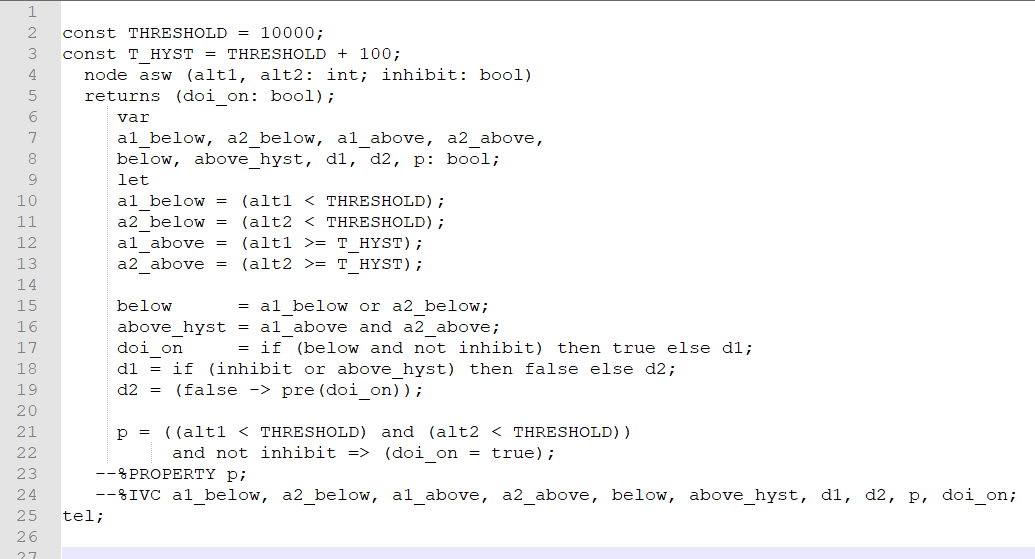
\includegraphics[width=\textwidth]{figs/exjk.png}
  %\vspace{-0.1in}
  \caption{An example of a LUSTRE program}
  \vspace{0.1in}
  \label{fig:exjk}
\end{figure}

%Inductive validity cores can be used for traceability from property to model elements and determining coverage of the model by a set of properties~\cite{Ghass17Cov}.  This facility can be used to automatically generate traceability and adequacy information (such as traceability matrices~\cite{fifarek2017nfm} important to the certification of safety-critical avionics systems~\cite{DO178C}.
%The IVC engine uses a our \ucalg algorithm to efficiently produce minimal or nearly minimal cores. As a side-effect, the IVC algorithm also minimizes the set of invariants used to prove a property and emits this reduced set to other engines.
To perform IVC analyses, we have extended \jkind with a set of IVC generation engines. When a property is
proved and IVC generation is enabled, our IVC engine
executes one of the {\ucalg, \bfalg, \ucbfalg}~algorithms \cite{Ghass16} to generate an (approximately) minimal IVC. This IVC generation engine is used to implement the \getivc\ procedure in  Algorithm \ref{alg:aivc}. For generating all minimal IVCs, we have added another engine to \texttt{JKind} that implements our online and offline algorithms.
%It worth mentioning that we could have employed the \ucbfalg ~algorithm for this purpose as well.
%One might say that since \ucbfalg ~guarantees minimality, it would help to the \aivcalg ~algorithm terminate more quickly.
%However, as we will show in the experiments, on the one hand, the \ucbfalg ~algorithm is very expensive. On the other hand, the \ucalg ~algorithm is not only fast, but it also generates \ivc s that are
%quite close to the \mivc s computed by \ucbfalg.

As previously discussed, one issue that needs to
be handled in any implementation of the \ucalg, \ucbfalg, and \aivcalg~algorithms involves the undecidability of the model checking problem;
in each iteration of Algorithms~\ref{alg:naive} and~\ref{alg:aivc} from Chapter \ref{ch:ivc}, we attempt to prove the property with a subset $S$ of the original model.  Although we know that $(I, T) \vdash P$, from Theorem~\ref{thm:minimal-hard}, the problem of determining whether or not any $S \subset T$ is adequate is undecidable.
%
Therefore, we have to set timeouts for the model checking algorithm for each iteration of the \aivcalg\ procedure.
In our implementation, we measure the time required to prove the property over the original model (\emph{proof-time}), and the time required to calculate the first
(approximate) IVC using \ucalg\ (\emph{\ucalg-time}).
The timeout we set for each iteration of the \ucbfalg\ and \aivcalg\ algorithms is ($30$ sec  $+\ 5\ \times$ (\emph{proof-time} $+$ \emph{\ucalg-time})).

If the \texttt{while} loop times out for $S$ in line 8 of Algorithm~\ref{alg:aivc},
we treat $S$ as an \emph{inadequate} set to ensure that all results support a proof.
In this case, line 13 will prune off $S$ and all
its subsets from the search space.  Since the timeout is used by both the brute-force
algorithm and the \aivcalg\ algorithm, minimality is only guaranteed if there
are no timeouts.  If a timeout occurs during computation, we report a warning to the user that our results are not guaranteed to be minimal.
It is important to note that by increasing the timeout, it is possible that
in some cases smaller IVCs can be generated, but the general problem will remain due
to the undecidability of the model checking problem.

To implement \bvcalg\ algorithm, a new tool is buit on top of \texttt{JKind}. In the implementation, basically, the \texttt{JKind} BMC engine has been hacked to emit the bounded cores after each step of transition relation unrolling. The user needs to provide a desired bound and timeout for this calculation.

The additional IVC engines integrated in \jkind are shown in Figure \ref{fig:ivcengines}.
Once IVC generation is activated, through $-ivc$ options, an approximately minimal IVC is generated. If \jkind has been called with $-all\_ivcs$, the IVC\_UC engine passes the first approximate MIVC to the All\_IVCs engine, where one of the all IVC generation algorithms will run depending on the provided configuration.

\begin{figure}
  \centering
  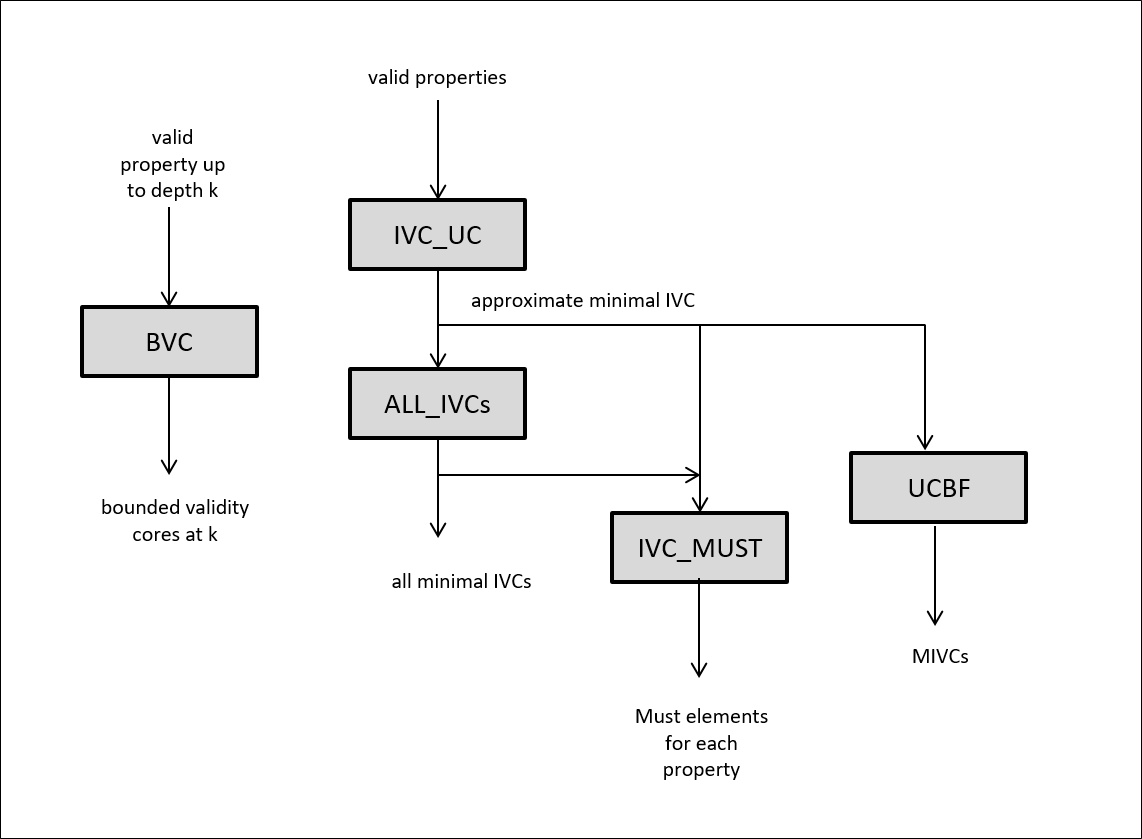
\includegraphics[width=0.8\textwidth]{ivceng.png}
  \caption{\jkind IVC engines}
  %\vspace{-1em}
 % \mike{Shrink figure vertically}
  \label{fig:ivcengines}
\end{figure}

\noindent There are three stand-alone tools implemented in \jkind:
\begin{itemize}
  \item BVC: this engine starts bounded model checking for a given bound within a specified timout. At the end of the process, it returns bounded validity cores.
  \item IVC\_MUST: $MUST$ computation comes for free after  $-all\_ivcs$ engine finds all the minimal MIVCs. The by-product of having all MIVCs are the $MUST$ elements, the intersection of all MIVCs. However, $MUST$ elements can be computed from one single (approximate) minimal IVC, as explained in Chapter \ref{ch:apps}. The IVC\_MUST engine can be called individually and as input it takes the output of IVC\_UC engine.
  \item UCBF: this is another stand-alone engine that takes the output of IVC\_UC engine and minimize the approximate MIVC to guarantee minimality.
\end{itemize}

To wrap up this section, we attach the outputs of the IVC engines for our running example (Figure \ref{fig:ucout}- \ref{fig:bvcout}).


\begin{figure}
  \centering
  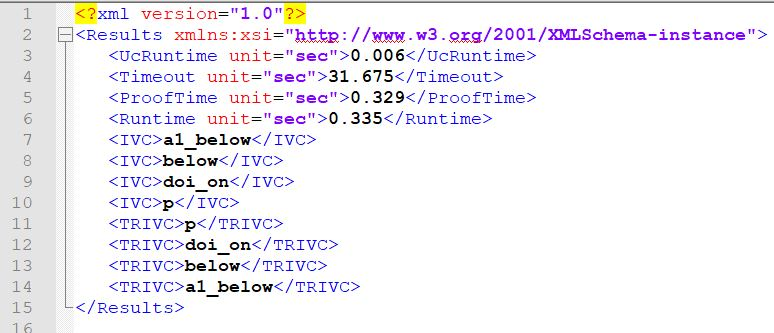
\includegraphics[width=0.9\textwidth]{figs/ucout.jpg}
  \caption{Sample output of IVC\_UC engine}
  %\vspace{-1em}
 % \mike{Shrink figure vertically}
  \label{fig:ucout}
\end{figure}

\begin{figure}
  \centering
  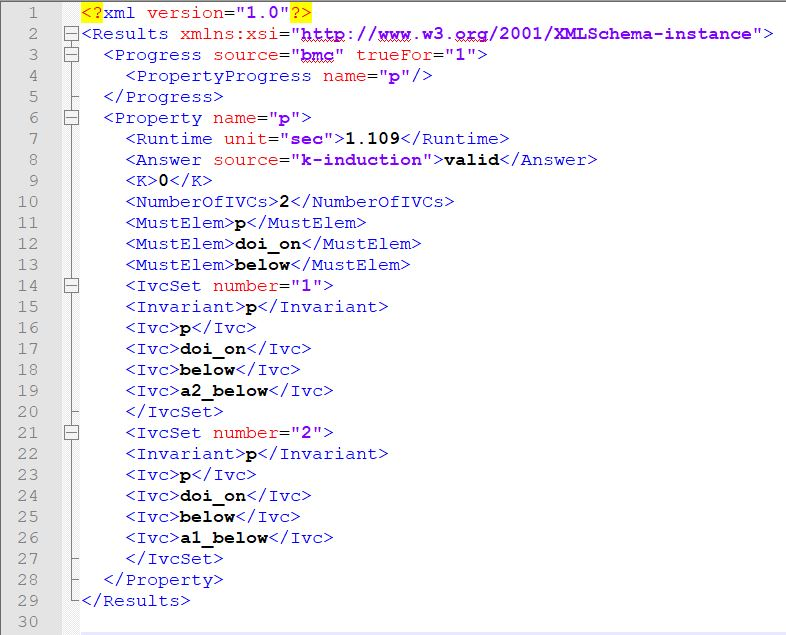
\includegraphics[width=0.9\textwidth]{figs/aivcout.jpg}
  \caption{Sample output of ALL\_IVCs engine}
  %\vspace{-1em}
 % \mike{Shrink figure vertically}
  \label{fig:aivcout}
\end{figure}

\begin{figure}
  \centering
  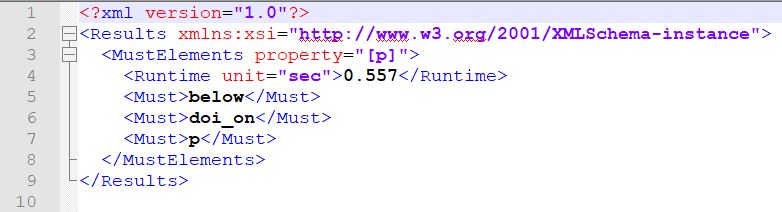
\includegraphics[width=0.9\textwidth]{figs/mustout.jpg}
  \caption{Sample output of IVC\_MUST engine}
  %\vspace{-1em}
 % \mike{Shrink figure vertically}
  \label{fig:mustout}
\end{figure}

\begin{figure}
  \centering
  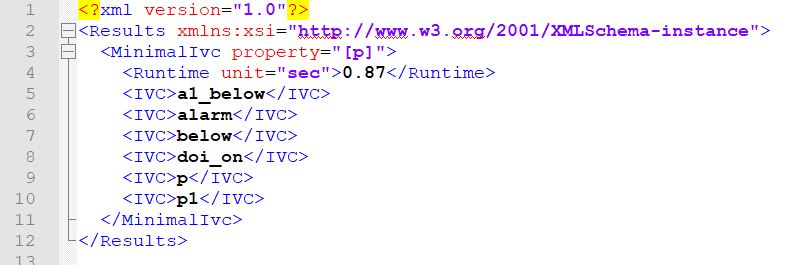
\includegraphics[width=0.9\textwidth]{figs/ucbfout.jpg}
  \caption{Sample output of UCBF engine}
  %\vspace{-1em}
 % \mike{Shrink figure vertically}
  \label{fig:ucbfout}
\end{figure}

\begin{figure}
  \centering
  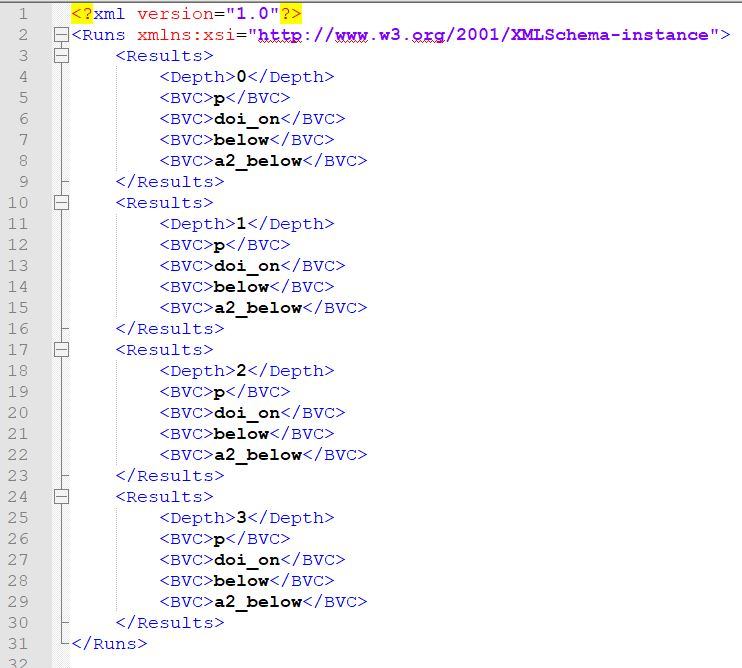
\includegraphics[width=0.9\textwidth]{figs/bvcout.jpg}
  \caption{Sample output of BVC engine for bound 4}
  %\vspace{-1em}
 % \mike{Shrink figure vertically}
  \label{fig:bvcout}
\end{figure}

\section{ Integration of {\sc JKind} and IVCs into Other Tools}

%\mike{Should we talk less (and less repetitively) about each table and use a chart that describes the jkind features used for each tool?}

\jkind is the back-end for a variety of user-facing applications. In this section, we briefly highlight a few and how they employ the features discussed previously.
%
\jkind  is developed in Java which makes it multi-platform and very easy to
integrate into other Java applications. Moreover, it comes with
\jkindapi package which contains utilities for creating \lustre
specifications, calling \jkind, processing \jkind results, graphically
displaying real-time results, and nicely formatting counterexamples.
Many of the applications in this section make heavy use of \jkindapi.
%
\subsection{Assume Guarantee Reasoning Environment}

 The {\em Assume Guarantee Reasoning Environment} (\agree)~\cite{cofer2012nfm,QFCS15:backes,hilt2013} is an open-source compositional verification tool that proves properties of hierarchically-composed models in the Architectural Analysis and Design Language (AADL) language.  %\jkind as the default model checker for AGREE.
%
%\application{Assume Guarantee Reasoning Environment}{Open Source}

\noindent \jkind is used as the default model checker for the Assume
Guarantee Reasoning Environment (\agree)~\cite{cofer2012nfm}. \agree
refers to both an embedded language annex in the Architectural
Analysis and Design Language (AADL) and to a plugin for the OSATE AADL
Integrated Development Environment. The \agree annex annotates the
AADL model with formal requirements, and the plugin reasons about
these requirements. The purpose of \agree is to model behavioral
requirements of an embedded system using formal assume guarantee
contracts. The plugin generates Lustre specifications that are checked
by \jkind.
%
\agree makes use of multiple \jkind features including smoothing and
interval generalization to present clear counterexamples, IVC to show
requirements traceability, and counterexample generation to check the
consistency of an AADL component's contract. \agree also uses \jkind
for test-case generation from component contracts.

\subsection{Specification and Analysis of Requirements}

The {\em Specification and Analysis of Requirements} (\spear) tool is an open source tool for prototyping and analysis of requirements~\cite{fifarek2017nfm}.  Starting from a set of formalized requirements, \spear uses \jkind to determine whether or not the requirements meet certain {\em properties}.  It uses IVCs to create a traceability matrix between requirements and properties, highlighting unused requirements, over-constrained properties, and other common problems. \spear also uses \jkind with smoothing for test case generation using the Unique First Cause criteria~\cite{whalen2006issta}.
%
\spear captures
requirements in a way that is backed by the formal semantics of
\lustre, which enables them to be analyzed using model checking to
ensure they are correct and consistent.

\spear uses \jkind to prove properties over requirements, and uses IVC
to create a traceability matrix between requirements and properties.
This quickly highlights unused requirements, over-constrained
properties, and other common problems. \spear also uses \jkind for
test case generation using the Unique First Cause
criteria~\cite{whalen2006issta} by creating {\em trap properties}.
Each trap property is expected to be falsifiable, but in such a way
that the counterexample has exactly the desired properties for a given
test case. \spear uses smoothing in \jkind to ensure the resulting
test cases are simple and understandable.


%\application{Static IMPerative AnaLyzer}{Open Source}
\subsection{Static IMPerative AnaLyzer}

The {\em Static IMPerative AnaLyzer} (\simpal) is a tool for
performing compositional reasoning over
software~\cite{wagner2017spin}. \simpal is based on \limp, a \lustre-like imperative language with extensions for control flow elements, global variables, and a syntax for specifying preconditions, postconditions, and global variable interactions of
preexisting components. \simpal translates \limp programs to an
equivalent \lustre representation which is passed to the \jkind to
perform assume-guarantee reasoning, reachability, and viability
analyses. The feedback from these analyses is used to refine the
program to ensure that the software functions as intended.

\jkind is also used by two proprietary tools used by product areas within Rockwell Collins.  The first is a {\em Mode Transition Table} verification tool used for the complex state machines which manage flight modes of an aircraft.
\jkind is used to check properties and generate tests for mode and transition coverage from \lustre models generated from the state machines.
IVCs are used to establish traceability, i.e., which transitions are covered by which properties.  The second is a {\em Crew Alerting System} MC/DC test-case generation tool for a proprietary DSL used for messages and alerts to airplane pilots.  Smoothing is very important in this context as test cases need to be run on the actual hardware where
timing is not precisely controllable. Thus, test cases with a minimum
of changes to the inputs are ideal.
%
%These state
%machines often have few states, but hundreds of possible transitions between
%states. There is a priority ordering to resolve conflicts between
%transitions, but this can make it hard to fully exercise the behavior
%of a state machine. The flight controls group has developed a
%particular graphical representation to manage this complexity.
%
%We have developed a tool which formalizes these state machine models.
%Trap properties are used to generate test cases exercising all transitions. Here IVCs are used when a trap property is {\em valid}, which means it failed to generate a test case. The IVC indicates which
%transitions are blocking the transition we wish to exercise in the
%test case. The tool presents all this information graphically to its
%users.

%\subsection{Applications}
%
%\subsubsection{MC/DC Test Case Generation}
%
%An engineering group at Rockwell Collins develops equations
%which determine which messages and alerts should be delivered to
%pilots. Certification for this system requires extensive test cases
%which must satisfy criteria such as the Modified Condition/Decision
%Coverage (MC/DC) metric. We have developed a tool which generates
%these tests by translating the equations into \lustre and generating
%MC/DC trap properties in \jkind. Smoothing is very important in this
%context as test cases need to be run on the actual hardware where
%timing is not precisely controllable. Thus, test cases with a minimum
%of changes to the inputs are ideal.
%
%\subsubsection{Model-based Fuzzing}
%
%As part of an ongoing DARPA program, Rockwell Collins is
%developing a tool for generating fuzz tests from system models. This
%tool takes a \lustre description of a system and uses \jkind to
%generate test cases which exercise different portions of the model.
%Effective fuzz testing requires a huge number of test cases which is
%not feasible to generate solely with a model checker. Instead, this
%fuzzing tool uses interval generalization in \jkind to generate
%generalized counterexamples which it then randomly samples at high
%speed. In fact, research in this area has recently expanded interval
%generalization to trapezoidal generalization which is strictly more
%general, but still allows very fast random sampling.
%
%
%\subsubsection{The \gryphon Framework}
%
%The Rockwell Collins \gryphon
% framework~\cite{miller2010cacm} translates Simulink models to various
% analysis tools for verification and testing. \gryphon uses the \lustre
% language internally which was the originally motivation for \kind
% (and eventually \jkind) to accept \lustre. As \gryphon is the only
% application in our list which does not directly integrate \jkind, it
% does not specifically use any features of \jkind. Still, features like
% smoothing and IVC have been successfully used in combination with
% \gryphon to great effect.
%
%
%
%
%
%
%
%
%
%
